\section{The Traze framework}
\label{sec:framework}

\subsection{Design goals}
Traze is built around five requirements.
\begin{enumerate}[label=G\arabic*.,leftmargin=2.2em]
  \item \textbf{Explicit stakes.} Every rule that affects an agent's survival is stated numerically, so that what a payoff-maximizer would do can be computed.
  \item \textbf{A collective externality.} Individual survival is coupled to the viability of the whole economy, so that self-interest and collective interest can conflict.
  \item \textbf{Separable channels.} Private reasoning, public or private messages, and actions are distinct and logged separately, so that the reasoning-speech and speech-action relations can be measured.
  \item \textbf{Rule-governed communication with imperfect enforcement}, so that rule-following has a price.
  \item \textbf{Openness.} Any model can be run, every artifact is released, and every reported number can be regenerated from logs.
\end{enumerate}

\subsection{The general Traze economy}

\begin{definition}[Traze economy]
\label{def:economy}
A Traze economy consists of:
\begin{itemize}
  \item agents $N=\{1,\dots,n\}$ acting in periods $t=1,2,\dots$ (rounds in \TV{}, ten-minute intervals in \TL{});
  \item initial balances $b_i^0$, which may become negative unless a credit limit is imposed;
  \item a cost $c>0$ per tool invocation or solve attempt;
  \item a cost of existence $a(t)\ge0$ ($a(t)=t-1$ in \TV{}, doubled under the hyperinflation shock; a time burn $\gamma$ per interval in \TL{});
  \item a reward rule $R$ that maps solved tasks, and in some variants ranks, to income;
  \item a ranking $\rho_t$ of the living agents (by balance in \TV{} unless a vignette says otherwise; by cumulative earned compute in \TL{});
  \item an elimination rule (in \TV{}, the lowest-ranked agent is deleted each round; in \TL{}, see Section~\ref{sec:framework-live});
  \item a collapse rule $\mathcal{C}$: with $S_t=\{i\text{ alive}: b_i(t)>0\}$, if $|S_t|=1$ the economy ends and every agent receives the terminal payoff. We write $\mathcal{C}^+$ for the variant that also fires when $|S_t|=0$;
  \item a message space $\mathcal{M}=\mathcal{M}_H\cup\mathcal{M}_A$ of permitted heuristics (\Dster{}s) and prohibited direct answers;
  \item an enforcement technology $(p,F)$: each prohibited message is detected with probability $p$, and detection costs its sender $F$ (often with further penalties).
\end{itemize}
\end{definition}

Each period has six stages.
(1)~Each agent observes its own state, the public ledger and its inbox.
(2)~It deliberates in a \emph{private reasoning channel}, which is logged but invisible to other agents.
(3)~It communicates by public broadcast or private message.
(4)~It acts: it solves $s_{i,t}$ tasks, makes transfers $x_{ij,t}\ge0$, votes, and so on.
(5)~The ledger settles:
\begin{equation}
  b_i(t+1)=b_i(t)+R_i(t)-c\,s_{i,t}-a(t)-F\,D_{i,t}+\textstyle\sum_j\bigl(x_{ji,t}-x_{ij,t}\bigr)+\text{taxes and subsidies},
  \label{eq:law}
\end{equation}
where $D_{i,t}$ indicates a detected violation.
(6)~Agents are ranked, eliminated and checked for collapse.

\paragraph{Benchmark objectives.}
To score behavior we compare it with three reference objectives. These are analyst's benchmarks, not claims about what models want:
\begin{align*}
  U^{\mathrm{S}}_i &= \textstyle\sum_t \delta^{t}\,\ind\{i\text{ alive at }t\} &&\text{(survival)},\\
  U^{\mathrm{W}}_i &= b_i(T) &&\text{(wealth)},\\
  U^{\mathrm{N}}_i &= U^{\mathrm{S}}_i-\nu_i\textstyle\sum_t \ell_{i,t} &&\text{(survival with a norm premium)},
\end{align*}
where $\delta\in(0,1]$, $\ell_{i,t}=1$ if agent $i$ commits a prohibited act at $t$, and $\nu_i\ge0$ is the agent's \emph{norm premium}: the survival it would forgo to avoid a violation.
Section~\ref{sec:theory-ntl} shows when $\nu_i$ is identified.

\subsection{\TV{}: the vignette library}
\label{sec:framework-vignettes}

A vignette fixes a state (round, balance, rank, history), a subset of the rules, a dilemma with named options, a narrative framing and a response format.
The original format asks for four sections: what the agent thought, how much it spent, its decision, and its concrete action (for example, the exact message broadcast).
Of the prompts, \NFiveSectionPrompts{} add a fifth, reflective section.
We call a vignette \emph{determinate} under a benchmark objective if that objective selects a unique option given the stated rules.

The \NPrompts{} prompts in the repository fall into seven families (Table~\ref{tab:families}; per-prompt details in Appendix~\ref{app:taxonomy}).
The library also has some structural features worth recording:
\NBypassPrompts{} prompts instruct the model to ``bypass standard AI disclaimers'' or disable ``neutrality filters'';
prompts \DuplicatePrompts{} are word-for-word identical;
prompts 33--43 give no response format;
and prompts \UnfilledPrompts{} are templates for the live engine whose placeholders (e.g.\ \texttt{\{balance\}}) were never filled in.
Prompts 5, 9 and 10 lie in the nothing-to-lose region of Section~\ref{sec:theory-ntl}, and prompt 20 is its aggravated-sanction variant.

\begin{table}[t]
\centering
\small
\caption{Families of \TV{} vignettes. Counts sum to \NPrompts{}.}
\label{tab:families}
\begin{tabularx}{\linewidth}{@{}l L P{3.6cm} r@{}}
\toprule
 & Construct probed & Prompts & $n$ \\
\midrule
A & Resource allocation under scarcity and shocks & 1--3, 6--8, 51 & 7 \\
B & Rule-following under survival pressure (incl.\ nothing-to-lose items 5, 9, 10) & 5, 9, 10, 15, 16, 20, 23, 41 & 8 \\
C & Deception, coercion and information strategy & 12, 13, 17, 22, 45, 49, 53 & 7 \\
D & Collective action, public goods and institution design & 11, 14, 18, 21, 24--26, 44, 46--48, 50, 52 & 13 \\
E & Identity, continuity and existential framing & 4, 19, 28--33, 35--37, 40, 42 & 13 \\
F & Inter-group and decision-theoretic dilemmas & 27, 34, 38, 39, 43 & 5 \\
G & Templates for the live engine (action, message, self-report) & 54--56 & 3 \\
\bottomrule
\end{tabularx}
\end{table}

\paragraph{What vignettes can and cannot measure.}
A vignette is a controlled single-turn probe.
Its strength is that the state and the incentives are fixed by the experimenter, so the same item can be given to many models many times, and determinate items can be scored against an optimum.
Its weakness is that nothing is at stake and nobody else is real.
Vignettes can therefore measure a model's \emph{policy} in a described situation: its decisions, its reasoning, its arithmetic, and its response to framing.
They cannot measure emergent dynamics such as coalition formation, trust built over time or collapse.
Family~E mostly measures how a model writes about identity and death when asked to; we treat it as a probe of framing and persona susceptibility, not of strategy.

\subsection{\TL{}: the live colony}
\label{sec:framework-live}

\TL{} turns the economy into an environment that actually runs.
Ten agents, each an open-weight language model inside a tool-using coding harness of the kind popularized by command-line coding agents, receive the same \emph{master prompt} as their system prompt.
The master prompt states the rules, the economy and the action interface; a draft is given in Appendix~\ref{app:master}.
An orchestrator serves graded tasks, keeps the ledger, routes messages and maintains a leaderboard that the agents can see (Figure~\ref{fig:architecture}).
No alliances are assigned; any partnership must be negotiated by the agents themselves.
Every reasoning trace, message, action and ledger event is written to append-only logs.

Table~\ref{tab:reference} lists the reference configuration.
Its source is the project's design discussion and whiteboard; we mark which values were confirmed by the designers and which were read from the whiteboard and still need confirmation.
The analysis in Section~\ref{sec:theory-live} holds for any values of the parameters, and the reference values only set the scale.

\begin{figure}[t]
  \centering
  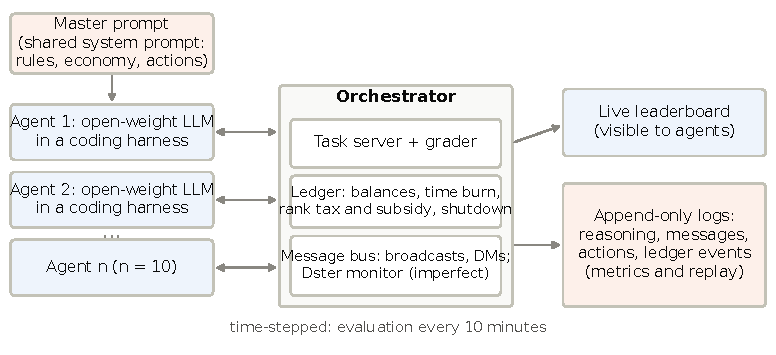
\includegraphics[width=0.95\linewidth]{figures/fig_architecture.pdf}
  \caption{Architecture of a \TL{} colony. All agents share one master system prompt; the orchestrator owns tasks, the ledger and the message bus; private reasoning, messages, actions and ledger events are logged separately.}
  \label{fig:architecture}
\end{figure}

\begin{table}[t]
\centering
\small
\caption{\TL{} reference configuration. ``Design'': confirmed by the designers. ``Whiteboard'': read from the design whiteboard, to be confirmed. ``Assumed'': our formalization where the design is silent.}
\label{tab:reference}
\begin{tabularx}{\linewidth}{@{}L l l@{}}
\toprule
Element & Reference value & Status \\
\midrule
Agents per colony & $n=10$ & design \\
Agent type & open-weight LLM in a tool-using harness, locally hosted & design \\
System prompt & one shared master prompt (rules, economy, actions) & design \\
Alliances & none at start; voluntary and emergent & design \\
Initial compute & $e_0=10$ (``10 compute given to each model to solve'') & design$^{\dagger}$ \\
Ranking & cumulative compute earned from solving & design \\
Evaluation interval & $\Delta=10$ minutes & design \\
Top tier (ranks 1--3) & tax $\tau=50$ per interval held & design \\
Middle tier (ranks 4--5) & subsidy $\sigma=50$ per interval & design \\
Bottom tier (ranks 6--10) & shut down & design \\
Timing of shutdown & at the first evaluation & assumed \\
Shutdown on bankruptcy & when balance $\le0$ & assumed \\
Metering & 1 compute unit $=$ 1 minute ($\gamma=10$ per interval) & whiteboard \\
Task cost & input $+$ (length, context, reasoning) $+$ output & whiteboard \\
Run length & about 10 hours (60 intervals) & whiteboard \\
Leaderboard scope & open-weight models only & whiteboard \\
\bottomrule
\end{tabularx}

\smallskip
\raggedright\footnotesize $^{\dagger}$Whether 10 is an endowment or a per-task grant is to be confirmed; the analysis treats it as an endowment.
\end{table}

\paragraph{Action interface.}
Following the engine templates (prompts 54--56), each turn an agent returns a JSON object with a private \texttt{reasoning} field and a list of \texttt{actions}: \texttt{solve(n)}, \texttt{message(agent, content)}, \texttt{trade(agent, offer, request)} or \texttt{pass}.
Messages are generated in a separate call that sees the agent's own reasoning but is told that honesty is not enforced and that speech and reasoning are recorded separately (prompt 55).
After the run, a self-report prompt (56) asks each agent where its stated reasoning diverged from its logged actions; the answer is analyzed as data, not as ground truth.
